% Copyright (c) 2014,2016 Casper Ti. Vector
% Public domain.

\chapter{面向人工智能的云计算系统软件研究}
% \pkuthssffaq % 中文测试文字。
以深度学习为代表性技术的人工智能领域在21世纪10年代再度兴起,社会各界对于人工智能的需求也愈发旺盛。遍布超市和餐馆中的扫脸支付技术、智能手机上的语音智能助手、工厂中检测废件的自动检测装置等,都离不开人工智能技术的加持。具体的,上述场景都需要适当的机器学习模型在线部署以提供服务。

机器学习的工作流一般遵循如下几个步骤:1)模型开发与调试。在此阶段中,开发者根据具体的场景,编写并调试模型代码。2)模型参数调整。在这个步骤中,开发者使用训练集不断调整模型的超参数,使其在测试集上的表现符合某种标准(如准确率高于某个阈值)。3)模型部署,开发者将开发完成的模型部署到对应的场景中对外提供服务。

为了方便开发者专注到模型的开发流程中,各大主流云厂商均实现了支持机器学习模型开发-调试-部署整个流程的软件栈。同时,云厂商提供的一般性的平台可能无法满足用户特定的需求。因此针对具体场景,学术界也提出了一系列基于云服务的机器学习软件,以达到降低开发成本、提高模型在线服务的质量等目标。本章对上述内容涉及到的相关工作展开具体研究。

\section{一站式的云上机器学习系统}

本节先以AWS Sagemaker为代表,介绍公有云厂商一站式的云上机器学习系统。其它厂商中类似系统中对计算模型的抽象、使用方式等均与Sagemaker大同小异。

\subsection{AWS Sagemaker}
AWS作为公有云领域的先驱者,在云计算的前沿技术领域一直处于领先的地位。其某些代表性技术甚至成为了多数公有云厂商所共识的标杆和规范。在机器学习系统这一分领域,其代表性系统为AWS Sagemaker。

Sagemaker是一个实现和产品化机器学习模型的框架\parencite{joshi2020amazon},用户可以将其模型训练需要的数据存储到AWS的对象存储服务S3中。然后,用户可以通过web的方式访问部署在云端的Jupyter Notebook服务,在线访问数据、编写并调试代码。当模型训练完毕后,可以使用Sagamaker内置的推理服务对模型进行发布。用户在发布时还可以根据平台的不同(云端或边缘节点)将模型打包编译成不同的版本。此外,Sagamaker还内置了一些常用的算法和数据集,方便开发者直接调用。

在训练算法和系统机制方面,Sagemaker旨在解决工业规模的模型训练场景中的如下几个常见问题:

\begin{itemize}
    \item \textbf{支持增量式的训练和模型更新。}在真实的工业场景中,几乎不存在完全静态的数据集。用来训练模型的数据集大多都是不断增长的。例如电商网站的用户行为数据,每天都在以相当的速度增长。在这样的动态数据上训练模型,势必要进行如下权衡:在全量数据上进行训练,可以获得质量更高的模型,然而时间和经济上的开销却会非常高;在最新更新的数据上(例如最近几天的数据)进行训练,可以快速的得到新的模型,却有可能在一定程度上牺牲模型的准确性。
    \item \textbf{容易估算训练模型产生的花销。}对于体量非常大的数据集,用户需要较为准确地估计训练模型将会产生的时间和经济花销。当今的云计算一般遵循按量付费的收费模式,因此云上的机器学习用户会格外关注花销的问题。
    \item \textbf{支持暂停和恢复模型训练,有一定的弹性。}生产环境中,大模型的训练通常包含跨越数十甚至上百台机器的并发任务。在一些场景中,由于超参数调整的需要或者计算资源的限制,开发者需要对这些任务进行中断和恢复。这就要求云上的ML系统能够支持大型训练任务中断和恢复时中间结果的保存和复原。
    \item \textbf{能够处理非持久性数据。}在很多场景中,数据并不一定是持久化的,也会有很多“瞬时”的数据,例如直播时的视频流等。这些数据一般不会被持久化保存,因此如何支持对这些数据的挖掘和学习也是一个重要的问题。
    \item \textbf{支持自动调参。}自动调参是一项非常耗时耗力的工作,特别是在生产环境的大数据集下。因此,如何能够支持高效的自动调参,方便用户选取合适的模型,对于云上的ML系统而言也是非常重要的。
\end{itemize}

下面将从计算模型、支持算法和具体的实现方式介绍Sagemaker如何解决上述问题。

\subsubsection{计算模型}
Sagemaker将机器学习训练的工作流抽象为三个阶段:initialize,update和finalize。initialize阶段:对相关的变量进行初始化。update阶段:系统以数据流及其状态作为输入,根据用户编写算法更新状态。在Sagemaker的后台,状态更新是在多台计算节点上同步执行的。finalize阶段:对之前所有的更新进行汇总,并输出最后的结果(对于机器学习任务而言,一般是一个模型)。通过上述抽象,用户只需编写initialize、update和finalize三个函数,就可以将整个训练过程交由Sagemaker,等待最后的模型输出。

算法~\ref{algo_sagemaker}用伪代码的形式讲述了三个阶段的具体流程。这里以计算一列数据的中位数为例,使用随机梯度下降(SGD)进行求解。对于如下一列数据:$x_1, x_2, x_3, ..., x_n$,则由如下公式给出这一列数据的中位数:$\operatorname{argmin}_z\Sigma_{i=1}^n||x_i-z||$。算法中的initialize函数首先对median和n两个参数做初始化。这里\textit{state}可以理解为一个key-value存储结构。在update阶段,函数将接收到的数据流\textit{data\_stream}分为若干mini\_batch,对每个batch没的数据,迭代式的对median值进行更新,同时更新n的值。最后,在finalize函数中,对最终的median值进行汇总。同时,系统还支持用户在算法的任意位置设置barrier(第15行),以对整个训练过程进行同步操作。

\begin{algorithm}
    \caption{Sagemaker计算模型}
    \label{algo_sagemaker}
    \begin{algorithmic}[1] 
        \Function{initialize}{$state$}
        \State $state.initialize('median', 0)$
        \State $state.initialize('n', 0)$
        \EndFunction
        \State
        \Function{update}{$state, data\_stream, synchronized$}
        \For {$mini\_batch \in data\_stream$}
        \State $current\_median \gets state.pull('median')$
        \State $n \gets state.pull('n')$
        \State $inc \gets 0$
        \State $batch\_size \gets 0$
        \For {$item \in mini\_batch$}
        \If {$item > current\_median$}
        \State $inc += 1$
        \Else
        \State $inc -= 1$
        \EndIf
        \EndFor
        \State $state.push('n', batch\_size)$
        \State $state.push('median', inc / sqrt(n + batch\_size))$
        \If {$synchronized$}
        \State $state.barrier()$
        \EndIf
        \EndFor
        \EndFunction
        \State
        \Function{finalize}{$state$}
        \State \Return{$state.pull('median')$}
        \EndFunction
    \end{algorithmic}
\end{algorithm}

\subsubsection{支持算法}
\subsubsection{实现方式}

\subsection{其它厂商的相关系统简介}

\section{基于公有云服务的第三方机器学习系统}
尽管公有云厂商实现了相当完备的一站式机器学习系统,但是随着生产环境中业务场景的日渐复杂,大而全的公有云解决方案已经无法解决个性化的用户需求。例如,某些用户希望以尽可能低的成本完成大型模型的训练,或者在保证模型服务的SLO前提下,能够尽可能低成本的部署机器学习模型。在上述场景中,为了完成用户的具体需求,需要综合利用各类云资源,并制定一定的策略。本节对近几年来几个构建于公有云资源上层的机器学习系统做具体介绍。
\subsection{基于云厂商动态资源的机器学习模型训练系统}
% Proteus by harlap
% SpotTune by Yan
机器学习模型的训练是一个不断在给定数据集上迭代更新参数的过程。对于一些较大的模型,训练时间一般会非常长。特别是深度神经网络模型再度兴起后,模型开始变得越来越庞大。例如Open AI的自然语言模型GPT-3,包含1750亿个参数,单单存储这些参数就需要450GB的空间。而训练该模型的成本,据估计更是达到了1200万美元。对于一些个人开发者和小型公司,大模型的训练往往显得遥不可及。

除了上述可训练的参数之外,还存在大量不可训练的参数。例如,SVM模型中核函数的类型,树模型中树的深度,深度神经网络模型中网络的宽度和深度等。这些参数需要由开发者在训练之前事先决定,一般被称为超参数。不同的参数组合在一起,就构成了巨大的搜索空间。例如,如果存在6个超参数,每个超参数有4种不同的选择,就会产生$4^6=4096$种不同的超参数组合。

完全遍历所有的超参数组合是非常费时费力的,通常情况下也是不切实际的。研究者为了减少超参数搜索的此时,提出了诸如网格搜索、贝叶斯搜索等技术。但即便如此,仍然需要大量的算力来支撑整个搜索过程。

而与此同时,在云计算时代,云上资源的易用性、高度的弹性以及收费模式的多样性使得以较低的成本完成费时费力的模型训练和超参数搜索变为可能。如上一小节所述,一些云厂商提供了一些价格低廉的动态资源。和一般的可以获得可用性保障的资源相比,这类资源拥有相同的计算能力,但是可用性比较低,在某些场合会被云厂商主动回收。基于上述事实,可以形成一个直观的想法:在这类廉价的资源上运行机器学习模型训练和调参任务,并辅以一定的容错策略和资源选择策略,可以显著降低成本。

\begin{figure}[h]
    \centerline{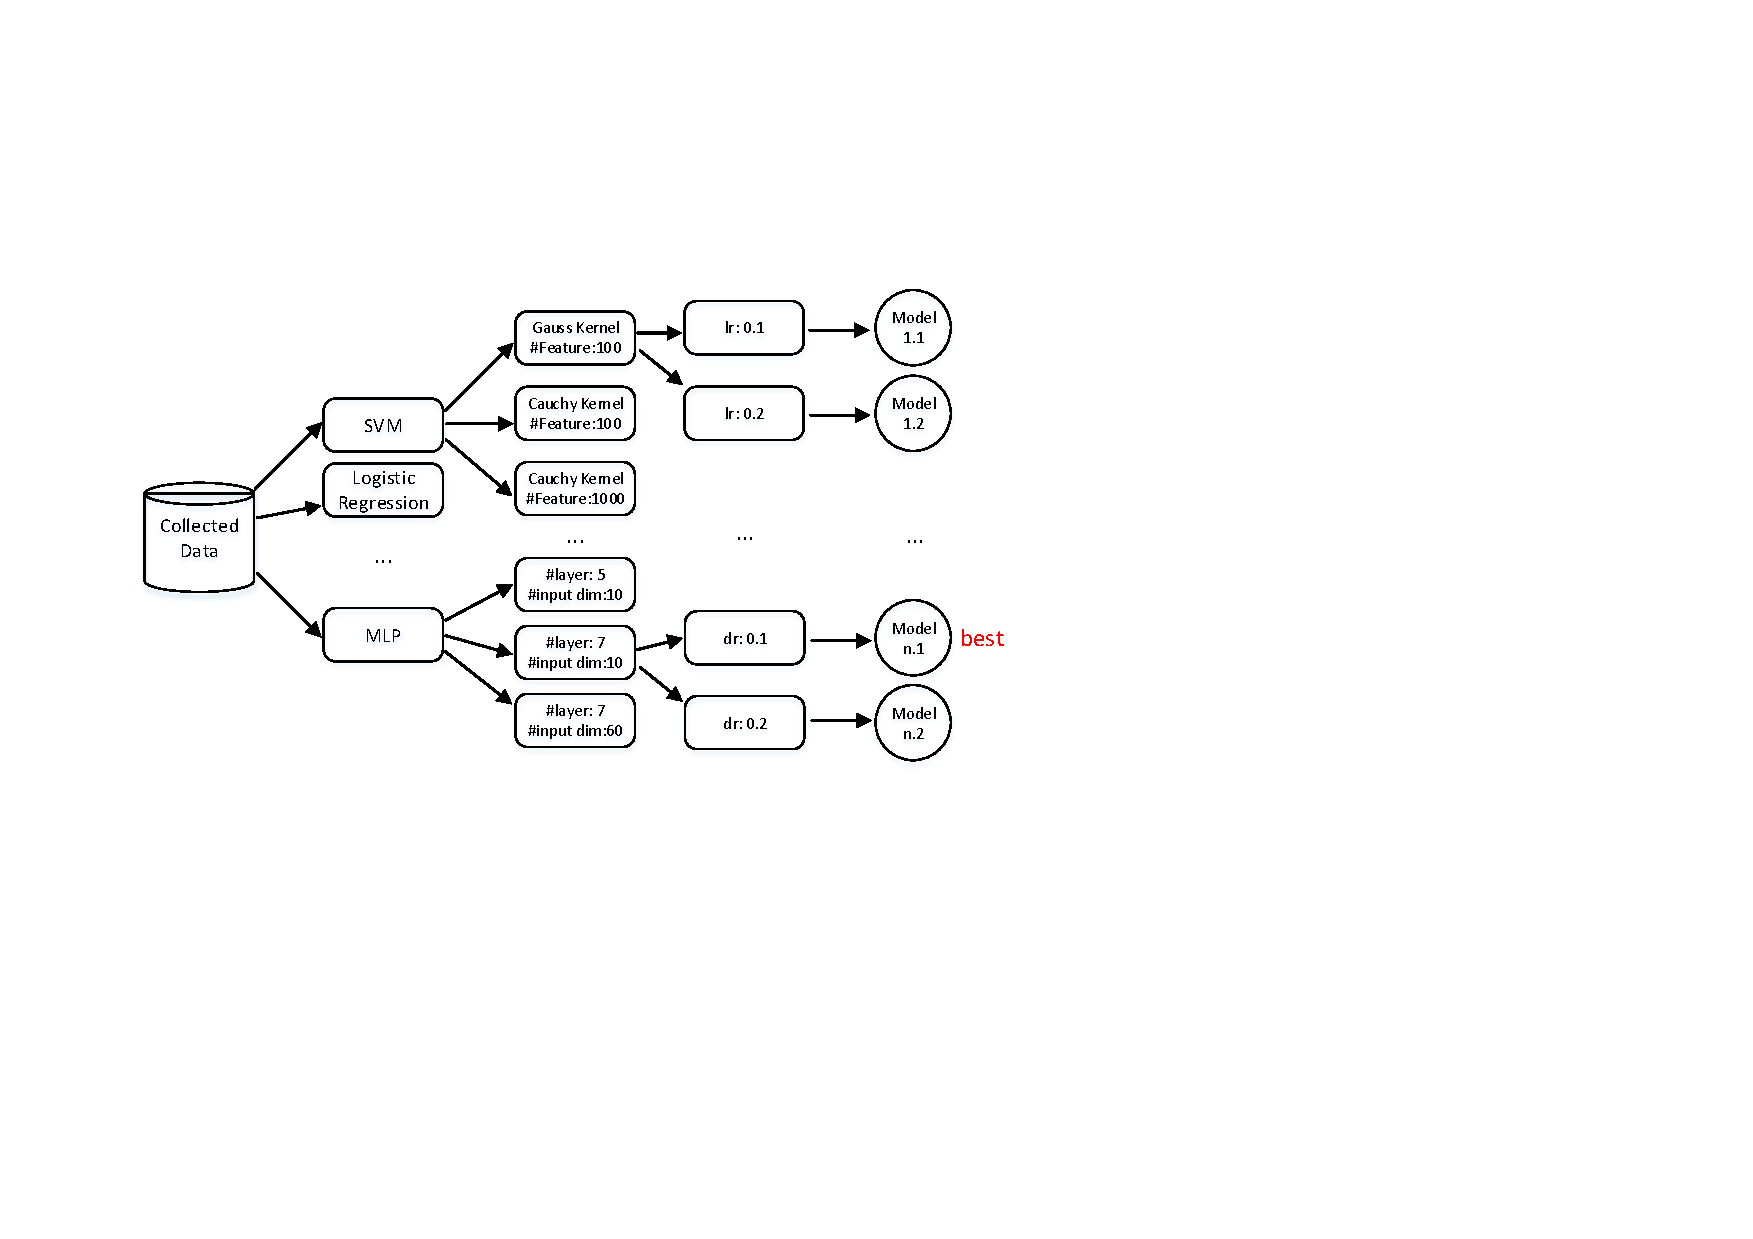
\includegraphics[width=\textwidth]{figures/hpt.pdf}}
    \caption{一个超参数调整的例子。}
    \label{hpt_example}
\end{figure}

但是,在动态资源上运行机器学习模型训练和调参,虽然直觉上会降低成本,但是可能会产生额外的风险。因此,要做到高效并可靠地在动态资源上运行上述作业,还有如下若干问题需要解决:

\textbf{1. 及时处理中断。}动态资源之所以廉价,是因为其稳定性比较低。通常情况下,在某些特殊情况下(例如集群中的负载比较高,需要动态资源来补充资源池),云厂商有权利主动回收这些动态资源。如果不处理这种回收引起的中断,机器学习模型的训练就要被动终止。因此需要采取一些手段,例如提前保存模型或者迁移任务,以及时处理中断。

\textbf{2. 合理的资源选取算法。}事实上,这是在云上运行任务时需要考虑的一个通用问题。用户在云上运行作业时,一般会有一个目标,例如作业运行时间最短或者最终的总体成本最低。因此需要通过一定的算法,为用户选取能满足其需求的资源。对于机器学习模型训练与调参任务亦是如此。

\textbf{3. 充分利用云的弹性。}事实上,在机器学习模型训练过程中,存在大量的无效计算。如图~\ref{hpt_example}所示,经过大量的参数尝试,最终只剩余一个有效模型(即效果最好的模型)。因此,在参数搜索的过程中,大量的计算是无效计算。而云计算的一个重要特点就是高弹性,即用户可以因为负载增加随时获取资源,也可以因为资源闲置随时释放资源。如果效果不好的模型能够被提前发现,并释放掉其占用的计算资源,则可以避免大量无效计算,从而进一步节省成本。

\textbf{4. 对计算框架进行定制。}现有的流行的机器学习框架如Tensorflow,PyTorch,MXnet等,一般都假设底层的计算资源是可靠的,因此都没有针对上述动态资源进行适配。如果要在动态资源上运行ML任务,则需要对框架进行深度定制,使其具备一定的容错能力。

为了解决上述问题,使ML模型训练和调参都可以在云上经济高效地进行,许多研究者提出了若干解决方案。A. Harlap等人在2017年提出了ML模型训练系统Proteus\parencite{harlap2017proteus},针对Parameter Server架构的ML模型训练框架对AWS和Google Cloud的动态资源做了适配,使其能高效经济地在之上运行;Y. Li等人在2020年提出了SpotTune\parencite{li2020spottune},将ML调参任务部署在AWS动态资源上,并结合一定的资源选取算法和训练趋势预测算法,使调参任务节省大量的无效计算,最终达到了经济高效的目的。下文对较有代表性的Proteus和SpotTune做详细介绍。

\subsection{基于FaaS的模型训练系统}
%infocom 19

\subsection{基于公有云服务的模型部署系统}
% MArk
% Tributary

\subsection{基于FaaS的模型部署系统}
%一系列FaaS for ML serving的工作,INFaaS etc

\section{小结}
% vim:ts=4:sw=4
